\documentclass{article}
\usepackage{amsmath}
\usepackage{amssymb}
\usepackage{graphicx}
\usepackage{listings}
\usepackage{xcolor}
\usepackage{url} % URLを扱うために必要
\usepackage{array} % 表のための機能を追加
\usepackage{booktabs} % 表のための上下の罫線とmidruleを提供
\usepackage{multirow} % 表のセルを複数行に結合するために必要
\usepackage{subcaption} % サブフィギュアを使用するために必要
\usepackage{float} % 図の位置制御のためのパッケージを追加

% LaTeXが\midruleを認識できない問題を解決するため、booktabsを再度確認
\makeatletter
\@ifpackageloaded{booktabs}{}{\usepackage{booktabs}}
\makeatother

% 日本語環境設定 (XeLaTeX用)
\usepackage{fontspec}
\usepackage{xeCJK}
\setCJKmainfont{Hiragino Sans} % macOSの日本語フォントに変更
\setCJKmonofont{Hiragino Sans} % モノスペースフォントも設定
\setmainfont{Hiragino Sans} % メインフォントにもUnicodeをサポートするフォントを設定
\setmonofont{Hiragino Sans} % モノスペースフォントにもUnicodeをサポートするフォントを設定

% リスティング設定
\lstset{
    language=Matlab, % デフォルト言語をMatlabに設定
    backgroundcolor=\color{white},
    basicstyle=\ttfamily\footnotesize,
    keywordstyle=\color{blue}\bfseries,
    commentstyle=\color{green!60!black},
    stringstyle=\color{red},
    numbers=left,
    numberstyle=\tiny\color{gray},
    stepnumber=1,
    numbersep=5pt,
    frame=single,
    breaklines=true,
    showstringspaces=false,
    captionpos=b
}

% --- 文書情報 ---

\title{数理モデル解析レポート:\\ロトカ・ヴォルテラ方程式における捕食者-被食者ダイナミクス}
\author{山北倫太郎}
\date{\today}

\begin{document}

\maketitle

\section{序論}
自然科学から社会科学に至るまで、私たちが直面する現象は多様な要因が複雑に絡み合った系として存在している。数理モデリングは、こうした複雑な現象から本質的な要素を抽出し、数学的に扱いやすい形式に定式化するプロセスだ。このアプローチにより、自然現象の理解だけでなく、将来予測や制御なども可能になる。

本レポートでは、生態系における捕食者と被食者の相互関係を記述する古典的モデルである「ロトカ・ヴォルテラ方程式」に焦点を当てる。このモデルは1920年代にアルフレッド・ロトカとヴィト・ヴォルテラによって独立に提案されたもので、シンプルな数式で生態系の動態を表現できる点が魅力的だ。

私が特にこのモデルに興味を持ったのは、非線形連立微分方程式という数学的に複雑な構造を持ちながらも、生物学的に明確な解釈が可能であるという点だ。講義で学んだ内容を応用して、このモデルの理論的な性質を解析し、さらにPythonを用いた数値シミュレーションを通じてその動態を視覚化する。これにより、抽象的な数式と現実の生態系現象との橋渡しを試みたい。

\section{理論的解析}

\subsection{ロトカ・ヴォルテラ方程式の導出}

ロトカ・ヴォルテラモデルは以下の連立微分方程式で表される[1, 2]:

\begin{align}
\frac{dx}{dt} &= \alpha x - \beta xy \\
\frac{dy}{dt} &= \delta xy - \gamma y
\end{align}

ここで、$x$は被食者(例:草食動物)の個体数、$y$は捕食者(例:肉食動物)の個体数を表す。各パラメータの生物学的意味は次の通りだ:

\begin{itemize}
\item $\alpha$: 被食者の内的自然増加率
\item $\beta$: 捕食者による被食者の捕食率
\item $\delta$: 捕食者が被食者を捕食することによる増殖効率
\item $\gamma$: 捕食者の自然死亡率
\end{itemize}

これらの方程式は、「食う・食われる」関係にある2種の生物の個体数変動を表現している。被食者は捕食者がいなければ指数関数的に増加し($\alpha x$)、捕食者との遭遇率に比例して減少する($-\beta xy$)。一方、捕食者は被食者を捕食することで増加し($\delta xy$)、自然死を通じて減少する($-\gamma y$)。

\subsection{解の存在と一意性}

ロトカ・ヴォルテラ方程式は、個体数が正である領域 $(x>0,y>0)$ において局所リプシッツ連続である[3]。これは、方程式の右辺が連続な偏導関数を持ち、有界な領域内では有界であることから確認できる。

そのため、\textbf{ピカール・リンデレフの定理(解の存在と一意性の定理)}により、この領域内の任意の初期値に対して、ただ一つの解(解軌道)が存在することが保証される[3]。これは数値シミュレーションを行う上での理論的基盤となる重要な性質である。

また、この性質により、異なる初期条件から出発した解軌道は決して交わらないことも保証される。つまり、系の未来の状態は初期条件によって一意に決定されるという決定論的な性質を持つ。

\subsection{平衡点分析}

システムの平衡点を求めるため、$\frac{dx}{dt} = 0$かつ$\frac{dy}{dt} = 0$となる点を求める[1]:

\begin{align}
\alpha x - \beta xy &= 0 \\
\delta xy - \gamma y &= 0
\end{align}

これを解くと、以下の2つの平衡点が得られる[2]:

\begin{enumerate}
\item 自明な平衡点: $(x, y) = (0, 0)$
自明な平衡点では両種が絶滅した状態を表す。

\item 共存平衡点: $(x, y) = (\frac{\gamma}{\delta}, \frac{\alpha}{\beta})$
共存平衡点では両種が安定して共存できる可能性がある状態を表す。
\end{enumerate}

\subsection{保存量の導出}

ロトカ・ヴォルテラ系の興味深い特性として、系に保存量が存在することが挙げられる[1, 2]。以下の関数$H(x,y)$を考える:

\begin{equation}
H(x,y) = \delta x - \gamma \ln x + \beta y - \alpha \ln y
\end{equation}

この関数の全微分を計算すると:

\begin{align}
\frac{dH}{dt} &= \frac{\partial H}{\partial x}\frac{dx}{dt} + \frac{\partial H}{\partial y}\frac{dy}{dt} \\
&= \left(\delta - \frac{\gamma}{x}\right)(\alpha x - \beta xy) + \left(\beta - \frac{\alpha}{y}\right)(\delta xy - \gamma y) \\
&= 0
\end{align}

したがって、$H(x,y)$は系の保存量(第一積分)となっている[2]。これは相平面上で軌道が閉曲線になることを意味し、捕食者と被食者の個体数が周期的に変動することを示している[1, 3]。

\section{Pythonによる数値実験}

\subsection{数値シミュレーションの実装}
\begin{lstlisting}
import numpy as np
import matplotlib.pyplot as plt
from scipy.integrate import solve_ivp

# 1. 微分方程式を定義する関数
# z = [x, y] は被食者と捕食者の個体数ベクトル
# t は時間、alpha, beta, delta, gamma はモデルのパラメータ
def lotka_volterra(t, z, alpha, beta, delta, gamma):
    """
    ロトカ・ヴォルテラ方程式を定義する。
    """
    x, y = z
    dxdt = alpha * x - beta * x * y
    dydt = delta * x * y - gamma * y
    return [dxdt, dydt]

# 2. パラメータと初期条件の設定
# 理論解析との比較のため、以下の値を用いる
params = {
    'alpha': 1.5,  # 被食者の内的増殖率
    'beta': 1.0,   # 捕食率
    'delta': 1.0,  # 捕食者の増殖効率
    'gamma': 3.0,  # 捕食者の内的死亡率
}
# 初期個体数
z0 = [10.0, 5.0] # [被食者の初期値, 捕食者の初期値]

# シミュレーション時間の設定
t_span = (0, 30)  # シミュレーション期間(0~30時間)
t_eval = np.linspace(t_span[0], t_span[1], 1000)  # 評価する時間点

# 3. solve_ivp を用いた数値積分
# args にパラメータをタプルで渡す
sol = solve_ivp(
    lotka_volterra, 
    t_span, 
    z0, 
    args=(params['alpha'], params['beta'], params['delta'], params['gamma']),
    dense_output=True, # 密な出力を有効化
    t_eval=t_eval      # 評価する時間点を指定
)

# 4. 結果のプロット
# フォント設定
plt.rcParams['font.family'] = 'sans-serif'
plt.rcParams['font.sans-serif'] = ['Hiragino Sans GB', 'Arial', 'Helvetica', 'Yu Gothic', 'Meiryo']

# Figure 1: 時間変化のプロット
plt.figure(figsize=(10, 6))
plt.plot(sol.t, sol.y[0], label='被食者 (x)')
plt.plot(sol.t, sol.y[1], label='捕食者 (y)')
plt.title('ロトカ・ヴォルテラモデル:個体数の時間変化')
plt.xlabel('時間 (t)')
plt.ylabel('個体数')
plt.grid(True)
plt.legend()
plt.savefig('time_series.png', dpi=300)
plt.show()

# Figure 2: 相平面のプロット
# 共存平衡点の計算
x_eq = params['gamma'] / params['delta']
y_eq = params['alpha'] / params['beta']

plt.figure(figsize=(8, 8))
plt.plot(sol.y[0], sol.y[1], label='軌道')
plt.plot(x_eq, y_eq, 'ro', label=f'平衡点 ({x_eq:.1f}, {y_eq:.1f})')
plt.title('ロトカ・ヴォルテラモデル:相平面図')
plt.xlabel('被食者個体数 (x)')
plt.ylabel('捕食者個体数 (y)')
plt.grid(True)
plt.legend()
plt.axis('equal')
plt.savefig('phase_plane.png', dpi=300)
plt.show()

# 以下は追加のコードで、平衡点と初期値を示した相平面図
plt.figure(figsize=(8, 8))
plt.plot(sol.y[0], sol.y[1], label='軌道')
plt.plot(x_eq, y_eq, 'ro', label=f'平衡点 ({x_eq:.1f}, {y_eq:.1f})')
plt.plot(z0[0], z0[1], 'go', label=f'初期値 ({z0[0]:.1f}, {z0[1]:.1f})')
plt.title('ロトカ・ヴォルテラモデル:相平面図(初期値と平衡点)')
plt.xlabel('被食者個体数 (x)')
plt.ylabel('捕食者個体数 (y)')
plt.grid(True)
plt.legend()
plt.axis('equal')
plt.savefig('phase_plane_with_initial.png', dpi=300)
plt.show()
\end{lstlisting}

\subsection{シミュレーション結果と考察}

数値シミュレーションの結果を以下の図に示す。

\begin{figure}[htbp]
  \centering
  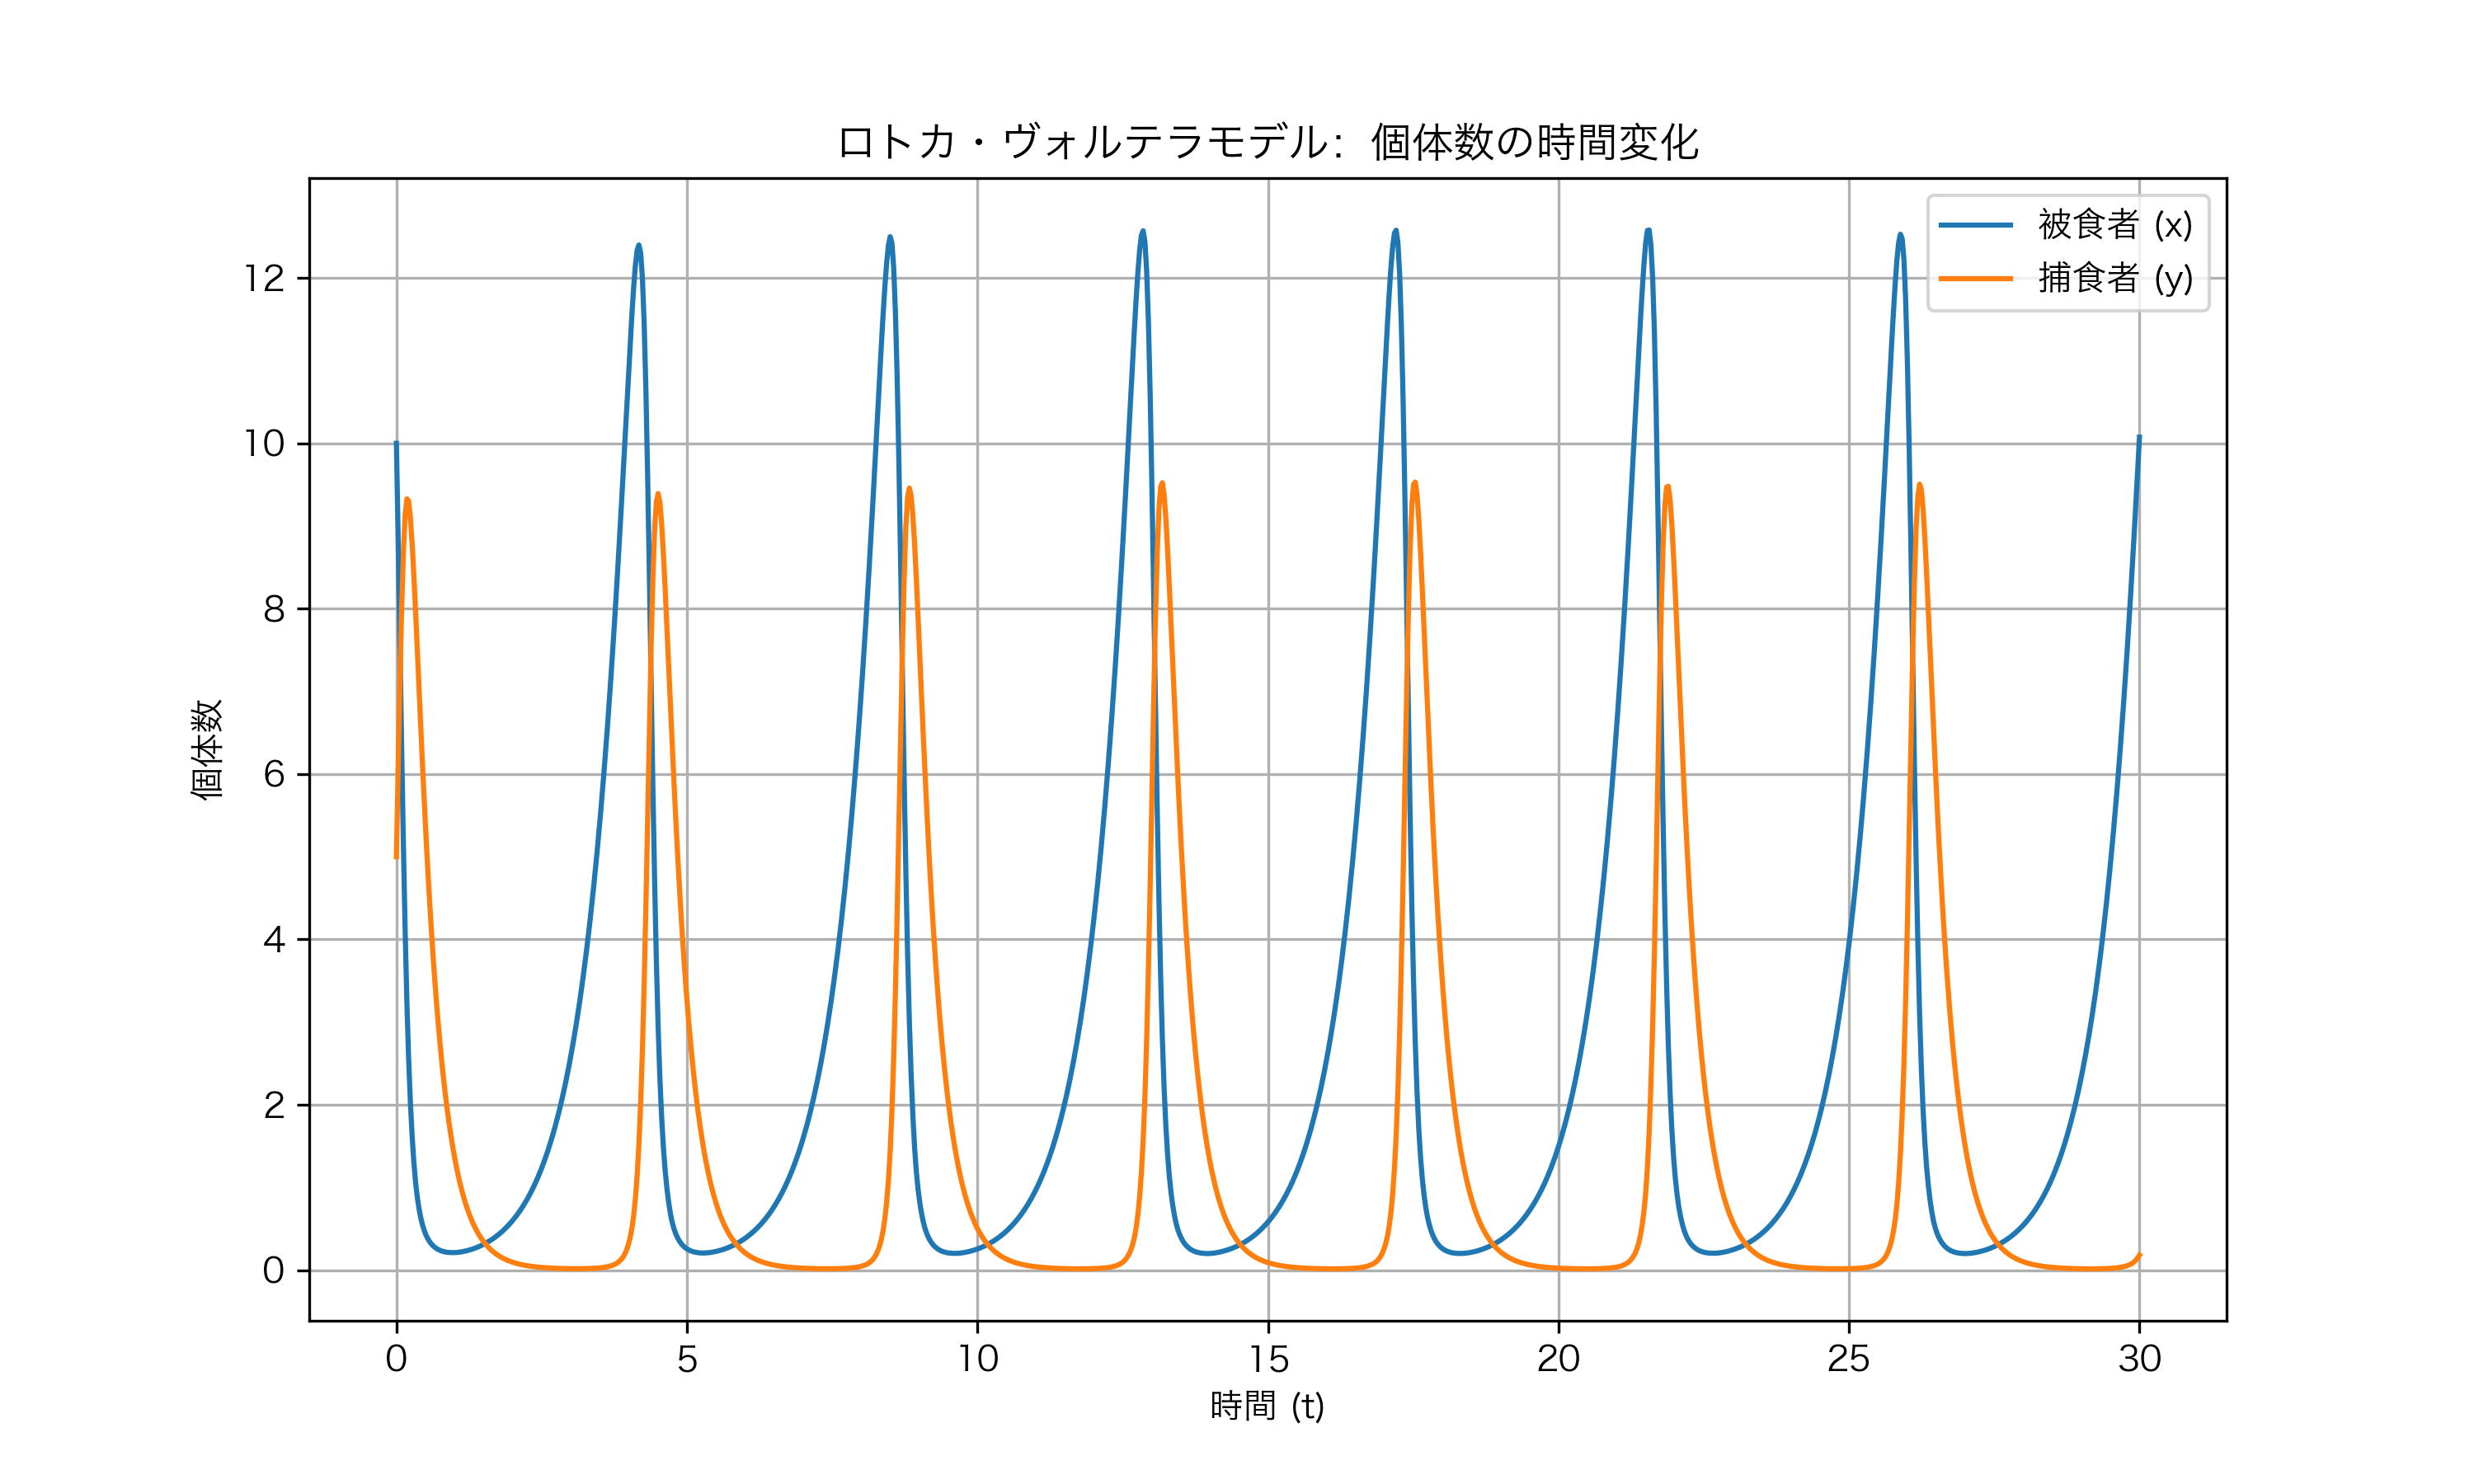
\includegraphics[width=0.9\textwidth]{time_series.png}
  \caption{ロトカ・ヴォルテラモデル:個体数の時間変化}
  \label{fig:time_series}
\end{figure}

図\ref{fig:time_series}は被食者と捕食者の個体数の時間変化を示している。グラフから明確に読み取れるように、両者の個体数は一定の位相差を持って周期的に変動している。被食者の個体数が増加すると、少し遅れて捕食者の個体数も増加する。捕食者が増えると被食者が減少し、そして被食者の減少に伴い捕食者も減少する。このサイクルが繰り返され、システムは安定した周期解を示している。特に注目すべきは、初期条件($x_0=10.0$, $y_0=5.0$)から出発した系が、理論解析で予測された通りの周期的振動を示している点だ。

\begin{figure}[htbp]
  \centering
  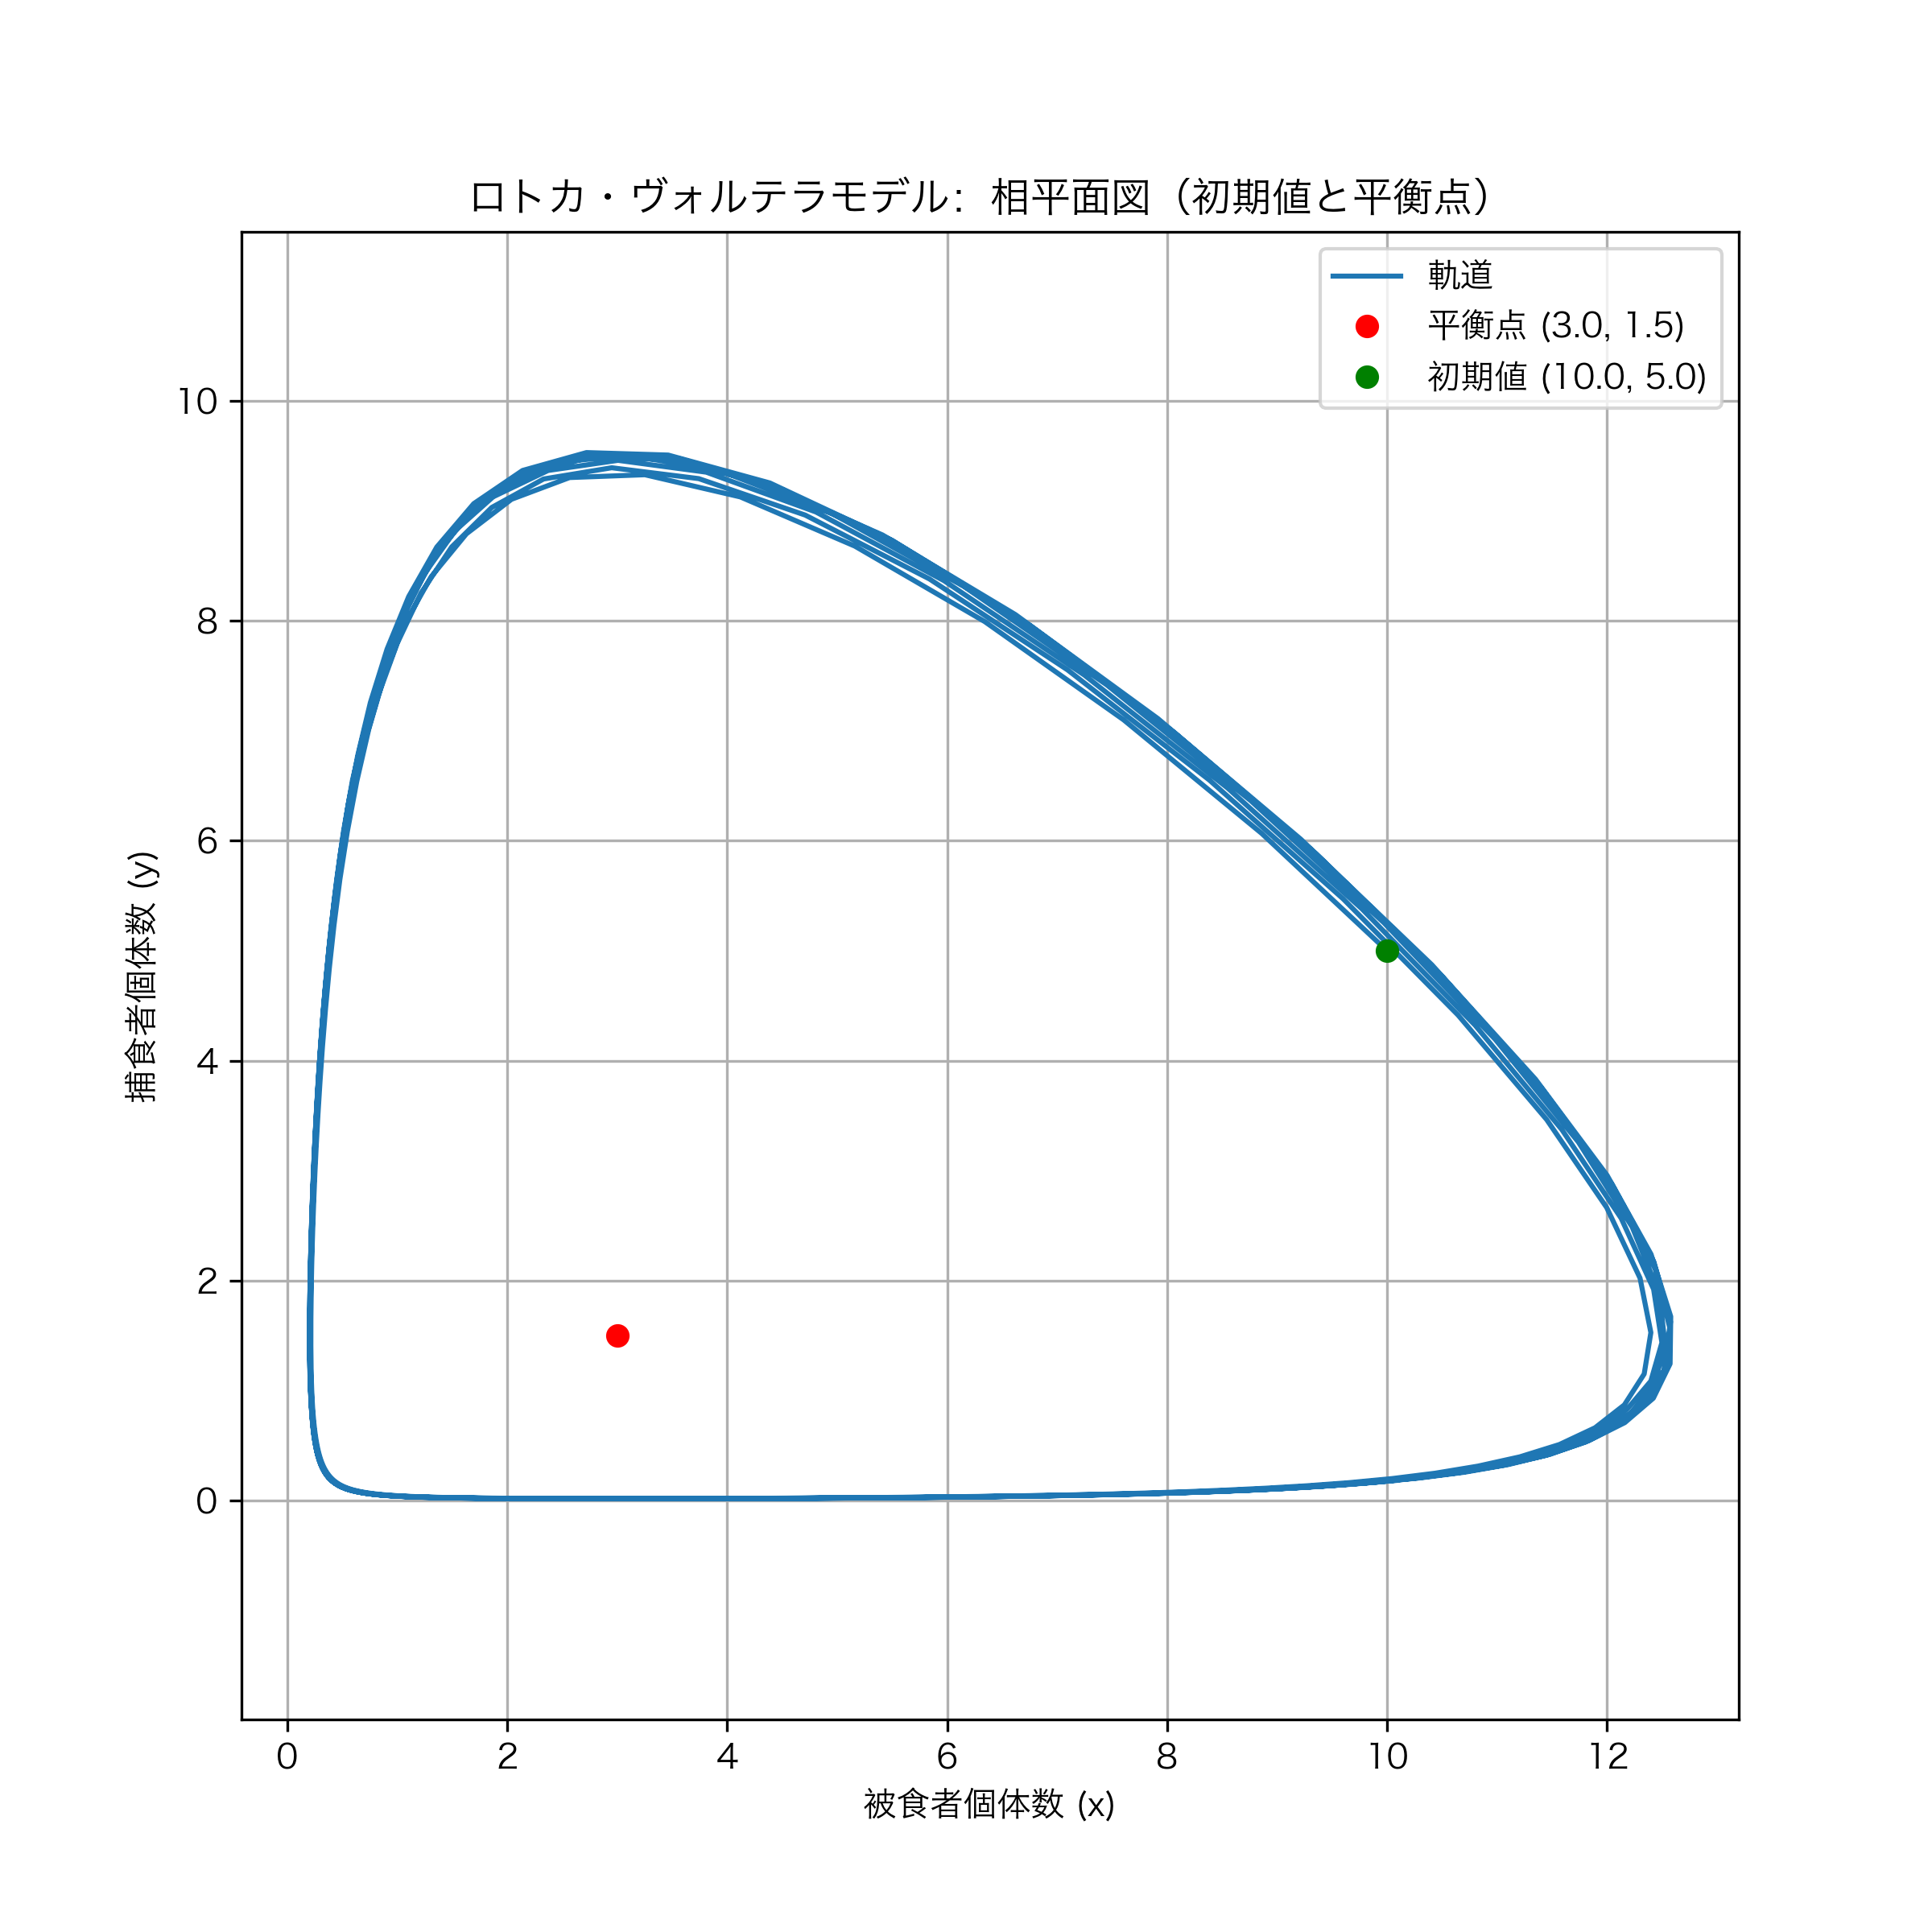
\includegraphics[width=0.8\textwidth]{phase_plane_with_initial.png}
  \caption{ロトカ・ヴォルテラモデル:相平面図(初期値と平衡点)}
  \label{fig:phase_plane}
\end{figure}

図\ref{fig:phase_plane}は被食者と捕食者の個体数の関係を相平面上に表した図である。理論解析で導出した共存平衡点($x_{eq}=3.0$, $y_{eq}=1.5$)が赤点で示されており、初期値($x_0=10.0$, $y_0=5.0$)は緑点で示されている。最も注目すべき点は、軌道が平衡点を中心とした閉じた曲線を描いていることだ。これは先ほど導出した保存量$H(x,y)$の存在を視覚的に確認できる証拠である。

相平面図からは、システムのダイナミクスが平衡点に収束するのではなく、平衡点の周りを周回し続けることが明確に見て取れる。これは平衡点が中立安定であることを示しており、小さな摂動が加わっても軌道は別の閉曲線に移るだけで、発散したり平衡点に収束したりすることはない。この特性は、現実の生態系でしばしば観察される捕食者-被食者サイクルの基本的なメカニズムを説明するものだと考えられる。

数値実験の結果は、理論解析で得られた洞察と完全に一致している。特に、系の保存量の存在により軌道が閉曲線になるという予測が、相平面図で明確に確認できた点は印象的だった。

\section{講義で学んだこと}

数理モデリングの講義を通じて、私は複雑な現象を数学的に記述することの力と限界の両方を学んだ。特に印象的だったのは、抽象的な数式から具体的な予測や洞察を引き出せることだ。ロトカ・ヴォルテラモデルのような単純な方程式でさえ、生態系の周期的変動という複雑な現象を説明できるという事実に驚かされた。

また、モデルの前提条件や限界を理解することの重要性も認識した。例えば、今回扱ったモデルでは環境収容力や捕食者の飽和効果などを無視しているが、より現実的なモデルを構築するにはこれらの要素も考慮する必要がある。モデルは現実の単純化であり、その前提を理解せずに結果を解釈すると誤った結論に至る危険性がある。

数値シミュレーションの実装を通じて、理論と計算の橋渡しの重要性も実感した。解析的に解けない問題でも、コンピュータを用いた数値計算によって視覚化し、直感的な理解を深めることができる。特にPythonのような高レベル言語とSciPyなどの科学計算ライブラリの組み合わせは、複雑なモデルを比較的容易に実装できる強力なツールだと感じた。

この講義で学んだアプローチやスキルは、生態学だけでなく、経済学、疫学、物理学など様々な分野で応用できると確信している。数理モデリングという方法論を通じて、現象の本質を捉え、将来予測や制御に活かすという視点は、今後の研究や実務に大いに役立つだろう。

\section{参考文献}

\begin{enumerate}
\item 犬伏正信. (2025). \textit{数理モデリング 講義資料 (mathmodel2025\_v1.pdf)}.
\item 巌佐 庸. (1990). \textit{数理生物学入門:生物社会のダイナミックスを探る}. HBJ出版局.
\item M. W. Hirsch, S. Smale, R. L. Devaney. (2017). \textit{力学系入門―微分方程式からカオスまで― (邦訳)}. 共立出版.
\end{enumerate}

\end{document}